\documentclass[11pt]{article}
\usepackage[margin=1in]{geometry}
\usepackage{amsmath,amssymb}
\usepackage{graphicx}
\usepackage{booktabs}
\usepackage{siunitx}
\usepackage[hidelinks]{hyperref}
\usepackage{caption}
\usepackage{authblk}
\usepackage{microtype}
\usepackage{enumitem}
\captionsetup{font=small,labelfont=bf}
\sisetup{detect-weight=true,detect-family=true}

\newcommand{\lres}{\lambda_{\mathrm{res}}}
\newcommand{\QL}{Q_L}
\newcommand{\rge}{\mathrm{RMS\text{-}RGE}}

\title{\bfseries ML-Driven Inverse Design of Microring Resonators for
Co-Packaged Optics / High-Bandwidth Optical Interconnects}

\author[1]{Md Shidul Islam Shihab\thanks{mdshidulislamshihab@gmail.com}}
\affil[1]{Department of Electronics \& Communication Engineering,
Khulna University of Engineering \& Technology (KUET), Khulna, Bangladesh}

\date{\today}

\begin{document}
\maketitle

\begin{abstract}
\noindent
Deep-learning inverse design of photonic components rests on an unresolved
disagreement. Liu \emph{et al.}\ [3] showed that a naive, non-tandem inverse
network can fail to converge when the design space is redundant; Chen and
Jiang [7] and Adibnia \emph{et al.}\ [9] reported naive inverse networks
converging acceptably in their own design spaces. This work resolves the
disagreement for a four-parameter, bus-coupled add-drop silicon microring
resonator by measuring both sides of it on one dataset with one set of
metrics. We build a dual-fidelity dataset of 1{,}150 labelled geometries over
ring radius, waveguide width, coupling gap and coupling length, with the
coupling coefficient obtained from 200 three-dimensional FDTD simulations of
the coupler alone and the ring response computed analytically, and we validate
the construction against a published, experimentally characterised device and
against 68 further independent FDTD runs.

The naive inverse network \emph{fails} the geometry-space criterion
($R^2 \ge 0.80$ on only one of four parameters) and \emph{passes} the
response-space criterion (closed-loop re-simulated error $3.669\%$, all
twenty test designs physically realisable). Both prior reports are therefore
correct, and were measuring different things. We explain why by counting
constraints: of four target quantities, resonance wavelength carries almost no
geometric information ($R^2 = 0.0078 \pm 0.0011$ across five seeds), free
spectral range fixes the round-trip length, and loaded $Q$ and insertion loss
both act through a single coupling phase $\theta$ --- two effective
constraints for four unknowns, leaving a two-dimensional degenerate family.

Three further results follow. First, geometry-space error does not predict
response-space error: across four models and three architecture families,
closed-loop error is proportional to $\theta$ error to within a factor
$1.20$, while the same ratio formed with $\rge$ varies by a factor $4.00$.
Second, physical realisability is architecture-dependent and is invisible to
both metrics --- Random Forest emits buildable geometries in $100\%$ of cases,
provably so by convexity, against $95.4\%$ for a plain network and $33.5\%$
for a tandem network. Third, a reproducible information bound computed from a
$10^6$-geometry response bank places the achievable $\rge$ at or below
$14.626\%$, which establishes that the $15\%$ objective threshold lies above
the information content of four scalar targets and that the measured shortfall
to $15.506\%$ is a model-and-data result rather than a fundamental limit.
Translating the designs into two co-packaged-optics scenarios, no method meets
any scenario's full specification; eleven of twelve failures involve resonance
placement, whose closed-loop error of $4.32$\,nm RMS exceeds a $\pm 2.0$\,nm
channel tolerance by a factor of two and a $\pm 0.4$\,nm tolerance by eleven.
Absolute resonance placement in this design space is beyond inverse design and
requires post-fabrication trimming.
\end{abstract}

\section{Introduction}

Inverse design asks for a geometry given a desired optical response. Where a
forward simulation is expensive, a natural approach is to train a surrogate on
simulated data and then invert it, and a substantial literature now does
exactly this for nanophotonic components [1,2]. Within that literature sits a
specific, unresolved disagreement about whether the simplest approach works.

Liu \emph{et al.}\ [3] argued that training a network to map response
directly to geometry fails when several geometries produce the same response:
the network is asked to fit a one-to-many relation and converges to an average
that is itself not a solution. Their remedy, the tandem network, trains the
inverse network through a frozen forward model so that the loss is measured in
response space, where the relation is single-valued. This argument is widely
accepted and widely cited.

Against it, two later studies report the naive approach working. Chen and
Jiang [7] inverse-designed a four-ring channel-dropping filter with two
independently trained networks --- no tandem --- and reported good convergence,
validating several designs by re-simulation. Adibnia \emph{et al.}\ [9]
likewise reported acceptable convergence for a direct inverse network. Neither
is a refutation of [3], and [3] is not a refutation of them, because the three
studies work in different design spaces and, critically, judge success by
different criteria: [3] reports geometric accuracy, while [7] and [9] report
how closely a re-simulated design reproduces the requested response.

No prior study resolves this for a microring resonator. Pal \emph{et al.}\ [6]
is the only work applying classical tree-based machine learning to microring
inverse design, on 462 finite-element samples, but their design space contains
no bus-coupling parameter at all and so cannot predict insertion loss or any
other coupling-dependent quantity --- the specifications that decide whether a
filter is usable in a co-packaged-optics (CPO) link. Torabi \emph{et al.}\
[12], the most recent and most dimensionally comparable study, defines the
$\rge$ metric adopted here but addresses a polymer-scale biosensor ring and
includes no classical-machine-learning baseline; it is also an unrefereed
preprint and is cited as such throughout. Valencia-Garz\'on \emph{et al.}\
[10] release a large all-pass dataset without modelling it.

This paper contributes the following.

\begin{enumerate}[leftmargin=1.6em,itemsep=2pt]
\item \textbf{A resolution of the disagreement}, measured on one dataset with
one protocol: the naive inverse network fails in geometry space and succeeds
in response space, so both camps are right. We give a closed-form reason, by
counting how many independent constraints four scalar targets actually impose.
\item \textbf{Evidence that geometry-space error is the wrong metric}, and a
physically motivated replacement that predicts response-space error across
architectures.
\item \textbf{A measurement of physical realisability as a first-class
result}, with a proof that one model family cannot violate the design box.
\item \textbf{A reproducible information bound} on inverse-design accuracy for
this design space, which separates model limitations from information limits.
\item \textbf{A controlled four-way comparison} of Random Forest, XGBoost, a
plain deep network and a tandem network on an identical split with identical
metrics, including a sample-efficiency characterisation --- the comparison
absent from [4,6,7,9,12].
\end{enumerate}

\section{Device, design space and methods}

\subsection{Device and parameterisation}

The device is a two-bus, four-port add-drop racetrack microring resonator on
silicon-on-insulator: silicon core of fixed height \SI{220}{nm}, SiO$_2$
cladding, fundamental TE mode only, scanned over
\SIrange{1500}{1600}{nm} with a nominal target of \SI{1550}{nm}. Both
couplers share a gap and coupling length, keeping the design space at exactly
four dimensions. Dispersive material models are used throughout; no constant
index is assumed. A racetrack rather than a circular ring makes the coupling
length a genuine continuous parameter, which is the degree of freedom absent
from [6], [10] and [12].

Table~\ref{tab:space} lists the four free parameters and the four targets. The
round-trip length is $L = 2\pi R + 2L_c$.

\begin{table}[t]
\centering
\caption{Design space and target quantities.}
\label{tab:space}
\small
\begin{tabular}{@{}llll@{}}
\toprule
Symbol & Parameter & Range & Note \\
\midrule
$R$    & ring radius      & \SIrange{5}{15}{\micro\metre} & spans FSR $\approx$ \SIrange{5.7}{18.2}{nm} \\
$w$    & waveguide width  & \SIrange{400}{500}{nm}        & single-mode strip on \SI{220}{nm} SOI \\
$g$    & coupling gap     & \SIrange{150}{350}{nm}        & near-critical to weakly coupled \\
$L_c$  & coupling length  & \SIrange{0}{3}{\micro\metre}  & $L_c = 0$ is a valid design point \\
\midrule
$\lres$ & resonance wavelength & nm & nearest to \SI{1550}{nm} \\
FSR     & free spectral range  & nm & adjacent-resonance spacing \\
$\QL$   & loaded quality factor & --- & $\lres/\mathrm{FWHM}$ \\
IL      & insertion loss        & dB & drop port, on resonance \\
\bottomrule
\end{tabular}
\end{table}

\subsection{Dual-fidelity dataset construction}

A full three-dimensional FDTD simulation of the complete ring was measured at
roughly \SI{35}{\hour} per sample, which puts a 1{,}000-sample dataset beyond
any realistic budget. A two-dimensional simulation runs in
\SI{149}{\minute} but returns a loaded $Q$ too high by a factor of
$11.3$, because it cannot represent vertical confinement.

The construction used instead simulates in three dimensions only the part of
the device that genuinely requires it. A single pass of the directional
coupler is simulated in 3-D FDTD to obtain the power coupling coefficient
$\kappa^2$; the ring response is then assembled analytically from coupled-mode
theory [13,14], with the effective and group indices taken from a 3-D mode
sweep and the propagation losses from a bend-loss sweep. The total cost is
approximately \SI{16}{\hour}.

A five-parameter model is fitted to the coupler simulations,
\begin{equation}
\kappa^2 = \sin^2\theta,
\qquad
\theta = \kappa_0(w)\,e^{-\gamma(w) g}
\left(L_c + B\sqrt{2\pi R/\gamma}\right),
\label{eq:theta}
\end{equation}
in which the gap and the coupling length enter \emph{only} through the single
phase $\theta$. Equation~\eqref{eq:theta} is the origin of the degeneracy
analysed in Section~\ref{sec:o6}, and $\theta$ is the quantity used as a
metric in Section~\ref{sec:metric}. The fitted $B = 1.0211$ is close to its
first-principles value of unity.

The coupler set was built in two stages by augmented Latin hypercube sampling:
48 points, then a further 152, for 200 in total. The extension widened the
$\kappa^2$ range from $0.0021$--$0.3138$ to $0.0019$--$0.4599$ and moved $B$
from $1.0425$ toward unity, with residuals flat across two and a half decades
and no evidence of $\sin^2\theta$ saturation.

The modelling dataset comprises 1{,}150 labelled geometries --- 1{,}000 from a
primary Latin hypercube design plus a 150-point supplementary batch covering a
sparse corner of the space --- split 805/172/173 into training, validation and
test sets with a fixed seed. The test set was used once.

\subsection{Validation of the construction}

\begin{table}[t]
\centering
\caption{Validation of the dual-fidelity construction. The out-of-sample
$\kappa^2$ tests are the coupler simulations performed during closed-loop
re-verification (Section~\ref{sec:metric}); they were not available to the fit.}
\label{tab:valid}
\small
\begin{tabular}{@{}llll@{}}
\toprule
Test & Quantity & Result & Criterion \\
\midrule
Published device [11] & FSR, \SI{440}{nm}$\times$\SI{220}{nm}, $R=\SI{20}{\micro\metre}$
  & \SI{4.4008}{nm} vs \SI{4.400}{nm} measured & $\le 10\%$ (O1) \\
                      & implied $n_g$ & $4.3443$ vs $4.3451$ & --- \\
$\kappa^2$ model      & 8-fold cross-validated MAPE & $3.36\%$, $R^2 = 0.9976$ & --- \\
$\kappa^2$ model      & 68 out-of-sample FDTD runs  & MAPE $1.23$--$5.16\%$, all within $10\%$ & --- \\
                      & systematic bias             & $-0.36$ to $+3.33\%$ & --- \\
Energy conservation   & $\kappa^2 + t^2$            & $1.0000$ on every run & --- \\
\bottomrule
\end{tabular}
\end{table}

Table~\ref{tab:valid} summarises three independent checks. The predicted free
spectral range of the fabricated device reported by Tang \emph{et al.}\ [11]
agrees with the measured value to within the precision of the published figure
(quoted as \SI{4.4}{nm}, i.e.\ $\pm 1.1\%$), well inside the $10\%$
requirement. Two caveats must accompany this validation. Only FSR is tested,
and FSR depends on group index and round-trip length alone, so the test
exercises the mode solver and the length convention and says nothing about the
coupling model, the bend-loss model, $\QL$ or IL. Further, the propagation
loss used in the analytic model (\SI{1.3}{dB/cm}) is itself taken from [11];
it does not enter the FSR prediction, so this particular comparison is
unaffected, but [11] is not an independent source for the loss model. We also
note that the loaded $Q \approx 3\times 10^5$ appearing in [11] is a stated
assumption in a scalability projection, not a measurement, and is therefore
not used here.

The $\kappa^2$ model was further tested on 68 coupler geometries that arose
during closed-loop re-verification and were never seen by the fit. Every one
fell within $10\%$, with a consistent positive bias of a few per cent that
should be reported as a known systematic.

\subsection{Models and protocol}

Four method families are compared, each in the forward and inverse direction,
on the identical split with identical metrics: Random Forest, XGBoost, a plain
feed-forward network, and a tandem network trained through the frozen forward
model. Tree models are evaluated with raw and normalised inputs. The forward
network architecture was selected by a 144-configuration grid search over
depth, width, learning rate and weight decay.

Two metric conventions require statement. Aggregate geometric error is the
root-mean-square relative geometric error
\begin{equation}
\rge = 100\% \times
\sqrt{\frac{1}{4}\sum_{p \in \{R,w,g,L_c\}}
\left(\frac{p^{\mathrm{pred}} - p^{\mathrm{target}}}{s_p}\right)^2 },
\label{eq:rge}
\end{equation}
with $s_p = p^{\mathrm{target}}$ for $R$, $w$ and $g$ following [12], and
$s_p = \SI{3}{\micro\metre}$, the range width, for $L_c$ --- necessary because
$L_c = 0$ is a valid design point at which a target-normalised relative error
is undefined. Per-parameter terms and the pure [12]-convention value over
$\{R,w,g\}$ are reported alongside every aggregate.

Closed-loop response error is measured by taking a model's predicted geometry
for each of twenty representative test targets, re-simulating the coupler in
3-D FDTD, reassembling the ring response, and comparing to the response
originally requested. The FDTD step is what makes this independent: feeding
predictions back through the fitted $\kappa^2$ model would merely replay the
model that produced the labels.

\section{Results}

Table~\ref{tab:score} summarises the outcome against the seven objectives
fixed before any modelling began. Three are met, three are not, and the
central one is resolved in the direction that the methodology document
anticipated as publishable. The objectives that are not met are reported as
measured, with the reason in each case identified rather than asserted.

\begin{table}[t]
\centering
\caption{Objective outcomes. O6 is the central contribution; O1--O5 and O7
exist to make its resolution credible rather than to stand as independent
results of equal weight.}
\label{tab:score}
\small
\begin{tabular}{@{}llp{7.4cm}@{}}
\toprule
& Outcome & Basis \\
\midrule
O1 dataset + validation & met & 1{,}150 geometries ($\ge 800$ required); FSR
agrees with [11] to within the published figure's precision, well inside
$10\%$ \\
O2 forward surrogate & \textbf{not met} & 2 of 4 targets; IL MAPE
$11.331 \pm 1.101\%$ against $\le 10\%$ over five seeds. Cause: small
denominators on a sub-decibel target, at $0.072$\,dB RMSE \\
O3 inverse accuracy & \textbf{not met} & $\rge = 15.506\%$ against
$\le 15\%$; closed-loop half met at $3.669\%$. Reachable in principle:
information bound $\le 14.626\%$ \\
O4 four-way comparison & met & all four families, identical split, every
metric, no omissions \\
O5 sample efficiency & met & XGBoost forward below 300 samples; network at
full size; naive network inverse at both \\
O6 one-to-many & \textbf{resolved} & geometry-space criterion fails (1 of 4
parameters at $R^2 \ge 0.80$), response-space criterion passes
($3.669\%$) --- both prior reports correct \\
O7 CPO translation & \textbf{not met} & 0 of 12 candidates, FDTD-verified;
11 of 12 failures involve resonance placement, which is physically out of
reach \\
\bottomrule
\end{tabular}
\end{table}

\subsection{The forward surrogate, and an unlearnable target}

\begin{table}[t]
\centering
\caption{Forward-direction accuracy on the held-out test set ($n = 173$).
Every method appears for every target. The best network is reported as a mean
over five training seeds, since the objective threshold is a hard bound and a
single run cannot distinguish a crossing from initialisation noise.}
\label{tab:fwd}
\small
\begin{tabular}{@{}lrrrrrrrr@{}}
\toprule
& \multicolumn{4}{c}{$R^2$} & \multicolumn{4}{c}{MAPE (\%)} \\
\cmidrule(lr){2-5}\cmidrule(lr){6-9}
Method & $\lres$ & FSR & $\QL$ & IL & $\lres$ & FSR & $\QL$ & IL \\
\midrule
DNN        & 0.0069 & 0.9993 & 0.9980 & 0.9969 & 0.158 & 0.561 & 3.205 & 10.346 \\
RF (raw)   & $-$0.0950 & 0.6892 & 0.9504 & 0.9342 & 0.166 & 17.288 & 12.640 & 25.351 \\
RF (norm)  & $-$0.0688 & 0.9920 & 0.9147 & 0.9072 & 0.164 & 2.730 & 17.340 & 27.483 \\
XGB (raw)  & $-$0.0837 & 0.9992 & 0.9634 & 0.9494 & 0.168 & 0.699 & 8.811 & 12.640 \\
XGB (norm) & $-$0.0795 & 0.9992 & 0.9808 & 0.9489 & 0.168 & 0.695 & 7.701 & 12.727 \\
\midrule
\multicolumn{9}{@{}l}{\itshape DNN over five seeds (42--46), mean $\pm$ s.d.:} \\
$\lres$ & \multicolumn{4}{l}{$R^2 = 0.0078 \pm 0.0011$} & \multicolumn{4}{l}{MAPE $= 0.158 \pm 0.000$\quad (0/5 seeds pass)} \\
FSR     & \multicolumn{4}{l}{$R^2 = 0.9993 \pm 0.0001$} & \multicolumn{4}{l}{MAPE $= 0.556 \pm 0.020$\quad (5/5 pass)} \\
$\QL$   & \multicolumn{4}{l}{$R^2 = 0.9982 \pm 0.0001$} & \multicolumn{4}{l}{MAPE $= 3.059 \pm 0.109$\quad (5/5 pass)} \\
IL      & \multicolumn{4}{l}{$R^2 = 0.9966 \pm 0.0003$} & \multicolumn{4}{l}{MAPE $= 11.331 \pm 1.101$\quad (1/5 pass)} \\
\bottomrule
\end{tabular}
\end{table}

The best forward model is the network, at $3.568\%$ mean MAPE across the four
targets against $5.323\%$ for the best XGBoost variant and $11.929\%$ for the
best Random Forest. Table~\ref{tab:fwd} reports all three required metrics for
every target and method.

Objective O2 required $R^2 \ge 0.90$ and MAPE $\le 10\%$ for at least three of
four targets. \textbf{Two of four are met, so O2 is not met.} Two points
about that verdict deserve care.

First, the verdict is reproducible, and it was measured as such. $\lres$ fails
on $R^2$ by an enormous margin and does so consistently; IL fails on MAPE at
$11.331 \pm 1.101\%$ against a $10\%$ bar, with only one seed in five passing.
A single training run is not a sound basis for a hard-threshold verdict, and
we report the distribution rather than a draw from it.

Second, IL's failure is a property of the metric and the target's scale, not of
the model's accuracy. IL is predicted to $0.072$\,dB RMSE with
$R^2 = 0.9966$. But the dataset's IL has a median of $0.524$\,dB, with
$48.3\%$ of rows below $0.5$\,dB and a minimum of $0.032$\,dB, so a constant
absolute error of $0.07$\,dB produces $13.7\%$ relative error at the median
and over $200\%$ at the extreme. Clearing a $10\%$ MAPE bar would require
absolute accuracy better than about $0.052$\,dB on a decibel quantity already
predicted to seven hundredths of a decibel. We report O2 as not met under the
criterion as defined, and note that $0.072$\,dB sits inside typical CPO
link-budget tolerance.

The resonance wavelength is not learnable by any method here. All four tree
variants return \emph{negative} $R^2$ --- worse than predicting the mean ---
and the network manages $0.0069$. The cause is sensitivity:
$\mathrm{d}\lres/\mathrm{d}R \approx 0.15$\,nm/nm, so placing a resonance to
within \SI{1}{nm} requires the radius to roughly \SI{7}{nm}, about one part in
$1.5\times10^4$ of the range. The consequence propagates: $\lres$ accounts for
almost all of the forward model's residual loss, so the 144-configuration grid
search was in effect ranking configurations on noise.

\subsection{The one-to-many question, resolved}
\label{sec:o6}

\begin{figure}[t]
\centering
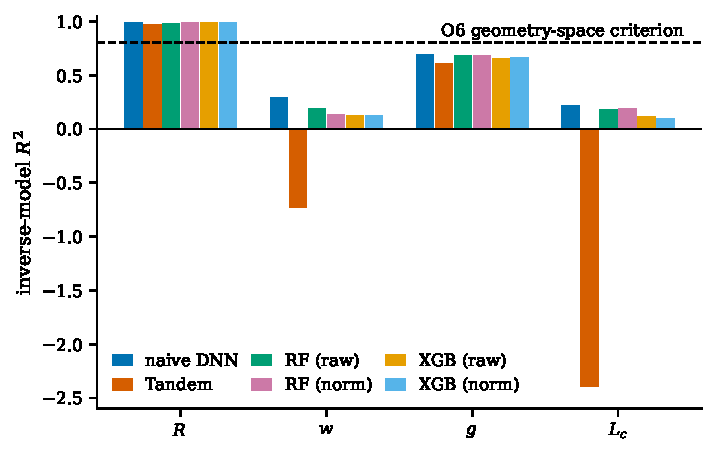
\includegraphics[width=\linewidth]{fig/fig1_o6_geometry_r2.pdf}
\caption{The geometry-space half of the one-to-many test. Only the ring radius
is recovered; width, gap and coupling length are not, for every method. The
dashed line is the $R^2 \ge 0.80$ criterion. The tandem network's negative
values for $w$ and $L_c$ indicate predictions worse than the test-set mean.}
\label{fig:o6}
\end{figure}

\begin{table}[t]
\centering
\caption{Inverse-direction accuracy, all methods on the identical test split.
$\rge$ is Eq.~\eqref{eq:rge}; per-parameter terms and the $\{R,w,g\}$-only
value are given as the metric convention requires. ``Buildable'' is the
fraction of test predictions lying inside the design box.}
\label{tab:inv}
\small
\begin{tabular}{@{}lrrrrrrr@{}}
\toprule
& \multicolumn{5}{c}{$\rge$ (\%)} & & \\
\cmidrule(lr){2-6}
Method & aggregate & $R$ & $w$ & $g$ & $L_c$ & $R,w,g$ only & Buildable \\
\midrule
naive DNN  & \textbf{15.506} & 2.841 & 5.321 & 14.144 & 26.930 & 8.878 & 95.4\% \\
Tandem     & 29.461 & 6.079 & 7.852 & 15.296 & 56.029 & 10.529 & 33.5\% \\
RF (raw)   & 16.039 & 5.942 & 5.741 & 14.378 & 27.460 & 9.574 & 100\% \\
RF (norm)  & 15.835 & 3.730 & 5.926 & 14.213 & 27.421 & 9.148 & 100\% \\
XGB (raw)  & 16.451 & 2.949 & 5.925 & 14.847 & 28.607 & 9.385 & 100\% \\
XGB (norm) & 16.546 & 2.986 & 5.941 & 14.687 & 28.900 & 9.308 & 100\% \\
\bottomrule
\end{tabular}
\end{table}

Objective O6 requires the naive inverse network to be judged against
\emph{both} criteria used by the two sides of the disagreement: a
geometry-space criterion of $R^2 \ge 0.80$, and a response-space criterion of
closed-loop re-simulated error.

\textbf{In geometry space the naive network fails.} Its per-parameter $R^2$
values are $0.9930$ for $R$, $0.2920$ for $w$, $0.6914$ for $g$ and $0.2166$
for $L_c$: one parameter of four clears $0.80$. Figure~\ref{fig:o6} shows
that this is not specific to the network --- every method recovers the radius
and no method recovers the other three.

\textbf{In response space the naive network passes, comfortably.} Re-simulating
its predicted geometries for twenty representative targets gives a
root-mean-square closed-loop response error of $3.669\%$, against a $20\%$
requirement, with all twenty predictions physically realisable. Per target:
$\lres$ $0.203\%$, FSR $0.980\%$, $\QL$ $4.037\%$, IL $3.594\%$.

This is the outcome in which the two literatures are simultaneously correct.
Liu \emph{et al.}\ [3] are right that the naive network does not recover the
geometry; Chen and Jiang [7] and Adibnia \emph{et al.}\ [9] are right that it
reproduces the requested response. The disagreement was never empirical.

\paragraph{Why: counting constraints.} The structure of the problem explains
the split exactly. Of the four targets, $\lres$ carries essentially no
geometric information, as Section~3.1 established. FSR fixes the round-trip
length $L = 2\pi R + 2L_c$. And $\QL$ and IL both depend on the coupling only
through $\kappa^2 = \sin^2\theta$, so they constrain the single phase $\theta$
of Eq.~\eqref{eq:theta} and nothing finer. Four targets therefore impose two
effective constraints --- one on $L$, one on $\theta$ --- on four unknowns,
leaving a two-dimensional family of geometries with indistinguishable
responses.

That prediction is quantitatively borne out. $L$ is dominated by $2\pi R$, so
$R$ is recoverable, and it is ($R^2 = 0.9930$). The remaining three parameters
enter only through $\theta$, and none is individually recoverable
($R^2 = 0.13$--$0.69$ across all methods). Direct confirmation: four
geometries with gaps spanning \SIrange{210}{270}{nm} and coupling lengths
spanning \SIrange{0.209}{2.353}{\micro\metre} share a loaded $Q$ of
$14\,659.8$ to the last digit. The naive network recovers $\theta$ itself to
$1.824\%$, with $96.5\%$ of its predictions within $5\%$ of the correct level
set. It is not failing; it is landing on the right level set and being scored
on its position along it.

\subsection{Geometry-space error does not predict response-space error}
\label{sec:metric}

\begin{figure}[t]
\centering
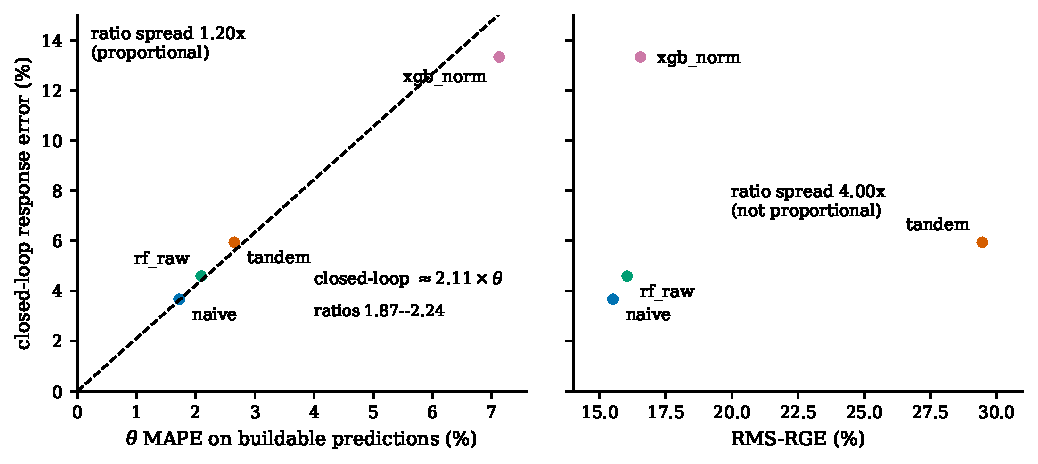
\includegraphics[width=\linewidth]{fig/fig2_theta_vs_closedloop.pdf}
\caption{Closed-loop response error against two candidate metrics, for the
four models whose predictions were re-simulated. Left: error in the coupling
phase $\theta$, evaluated on buildable predictions so that the two axes cover
the same designs. Right: $\rge$. The ratio of closed-loop error to $\theta$
error is constant to within a factor $1.20$; formed with $\rge$ it varies by a
factor $4.00$.}
\label{fig:metric}
\end{figure}

\begin{table}[t]
\centering
\caption{Closed-loop re-verification, four models, twenty targets each. All
clear the $20\%$ response-error bar. $\theta$ error is evaluated on buildable
predictions, matching the designs over which closed-loop error is measured.}
\label{tab:cl}
\small
\begin{tabular}{@{}lrrrrrrr@{}}
\toprule
Method & $\rge$ (\%) & $\theta$ err.\ (\%) & \multicolumn{4}{c}{closed-loop error, per target (\%)} & RMS (\%) \\
\cmidrule(lr){4-7}
 & & & $\lres$ & FSR & $\QL$ & IL & \\
\midrule
naive DNN  & 15.506 & 1.723 & 0.203 & 0.980 & 4.037 & 3.594 & \textbf{3.669} \\
RF (raw)   & 16.039 & 2.095 & 0.208 & 2.994 & 4.058 & 5.011 & 4.589 \\
Tandem\textsuperscript{$\dagger$} & 29.461 & 2.654 & 0.190 & 0.745 & 4.980 & 7.110 & 5.936 \\
XGB (norm) & 16.546 & 7.129 & 0.165 & 0.970 & 14.684 & 15.382 & 13.329 \\
\bottomrule
\multicolumn{8}{@{}l@{}}{\footnotesize\textsuperscript{$\dagger$}Over the 8 of 20 predictions that were buildable; see Section~\ref{sec:build}.}
\end{tabular}
\end{table}

Section~\ref{sec:o6} showed that geometric error and response error disagree
about whether a model works. Table~\ref{tab:cl} shows that they also disagree
about which models work, and by how much.

The naive network and XGBoost (normalised) differ by $1.04$ percentage points
in $\rge$ --- $15.506\%$ against $16.546\%$, a difference a reader would
reasonably call negligible. In closed loop they differ by a factor of
$3.6$: $3.669\%$ against $13.329\%$. Had only $\rge$ been measured, these two
models would have been called equivalent, and the conclusion would have been
wrong by nearly a factor of four on the quantity that determines whether a
design works.

The degeneracy suggests why, and $\theta$ makes it measurable. An error that
moves along a $\theta$ level set yields a different valid design; one that
moves across it yields a wrong response. Figure~\ref{fig:metric} tests this
on the four models whose predictions were re-simulated. Closed-loop error is
proportional to $\theta$ error, with the four ratios spanning
$1.87$--$2.24$, a factor of $1.20$. The same ratios formed with $\rge$ are
$0.20$--$0.81$, a factor of $4.00$.

Two features of that comparison matter for its strength. The first is that
model family is controlled: Random Forest (raw) is an ensemble method with
$\theta$ error $2.095\%$ and lands at $4.589\%$, beside the network's
$3.669\%$ and far from XGBoost's $13.329\%$. Within the tree family alone,
$\theta$ error varies by a factor $3.4$ and closed-loop error by $2.9$, while
$\rge$ differs by $3\%$ --- so there is no architecture explanation available.
The second is that ordering alone would not have discriminated: $\rge$ happens
to rank three of these four models correctly. What it cannot do is say how
much worse one is than another, which is what a design metric is for.

\subsection{Physical realisability}
\label{sec:build}

\begin{figure}[t]
\centering
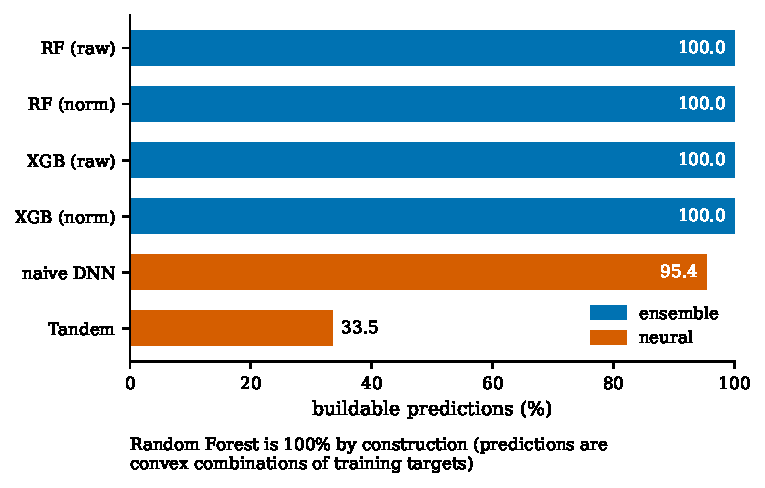
\includegraphics[width=0.74\linewidth]{fig/fig5_buildable.pdf}
\caption{Fraction of test-set predictions lying inside the design box. The
distinction is architectural, and invisible to both metrics of
Section~\ref{sec:metric}.}
\label{fig:build}
\end{figure}

Neither $\rge$ nor $\theta$ error detects a prediction that cannot be
fabricated, and the differences between architectures here are large.

The tandem network produced unbuildable geometries for twelve of the twenty
closed-loop targets: eleven with negative coupling length, down to
\SI{-0.881}{\micro\metre}, and one with a width of \SI{397.8}{nm}. Over the
full test set its buildable fraction is $33.5\%$. The mechanism is visible in
its loss: the tandem network is penalised only through the frozen forward
surrogate, which will evaluate $L_c = \SI{-0.88}{\micro\metre}$ and return a
plausible response. Nothing in the objective encodes that the design space has
edges. The naive network, which regresses against real geometries and is
therefore pulled toward a region where all targets are valid, leaves the box on
$4.6\%$ of the test set.

Both tree families produced buildable geometries in every case. For Random
Forest this is guaranteed rather than fortunate: its prediction is a mean of
leaf values and hence a convex combination of training targets, so it lies in
their convex hull, and the design box is convex. Gradient boosting is additive
rather than convex and carries no such guarantee, but violated the box
nowhere here.

The practical consequence is that $\theta$ error and realisable fraction are
complementary and both are needed; neither subsumes the other. The tandem
network illustrates why. On its buildable predictions its closed-loop error is
$5.936\%$, better than XGBoost's, and its $\theta$ error is a respectable
$2.654\%$. Judged on those numbers alone it looks like a competitive model.
Sixty per cent of its designs cannot be made.

\subsection{Method comparison and sample efficiency}

\begin{figure}[t]
\centering
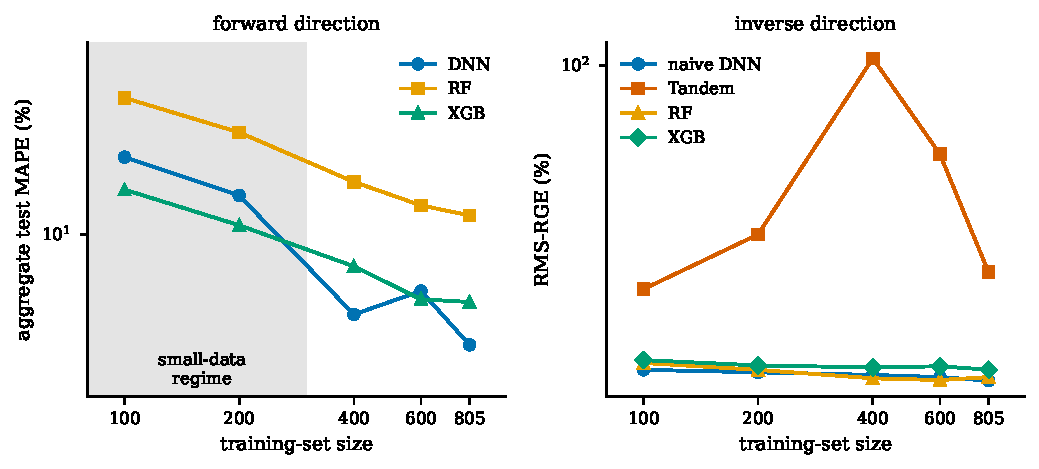
\includegraphics[width=\linewidth]{fig/fig3_sample_efficiency.pdf}
\caption{Sample efficiency. Left: in the forward direction XGBoost is more
accurate below about 300 training samples and the network overtakes it by the
full dataset. Right: in the inverse direction the naive network is best at
every size, and the tandem network is unstable, peaking at $104.3\%$ at 400
samples.}
\label{fig:sample}
\end{figure}

In the forward direction, XGBoost is the most accurate method in the
$\le 300$-sample regime, at $13.030\%$ mean aggregate MAPE over sizes 100 and
200 against the network's $17.465\%$; at the full 805-sample training pool the
network is most accurate, at $3.568\%$. In the inverse direction the naive
network is lowest at both ends --- $16.411\%$ mean $\rge$ in the
$\le 300$-sample regime and $15.506\%$ at full size.

The crossover is worth stating plainly because it bears on practice: for a
photonic design problem where each label costs hours of simulation, a
gradient-boosted tree is the better forward surrogate until a few hundred
samples have been gathered. Pal \emph{et al.}\ [6] drew their result from 462
samples and Torabi \emph{et al.}\ [12] from 2{,}500, so this range spans the
operating point of the closest published work.

The tandem network's inverse curve is not a learning curve at all: $26.6\%$,
$36.8\%$, $104.3\%$, $59.2\%$, $29.5\%$ across the five sizes. This is
consistent with the box-escape mechanism of Section~\ref{sec:build}; with
nothing anchoring predictions inside the design space, where the network
wanders is largely a function of initialisation and data.

A final observation on metric dependence. Ranking parameter difficulty by mean
$R^2$ gives $L_c > w > g > R$, hardest first; ranking by mean $\rge$
contribution gives $L_c > g > w > R$. The two orderings disagree on $w$
against $g$. Under either, the coupling gap is \emph{not} the hardest
parameter --- the coupling length is, with mean $R^2 = -0.2645$ --- which
refutes the hypothesis that $g$ would dominate by analogy with [6]'s finding
for radius.

\subsection{An information bound}

\begin{figure}[t]
\centering
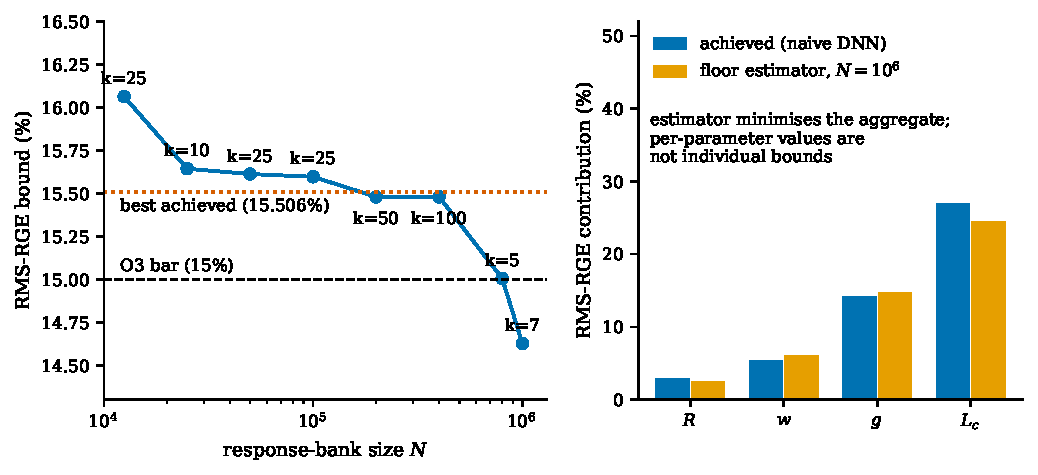
\includegraphics[width=\linewidth]{fig/fig4_information_floor.pdf}
\caption{Left: the information bound against response-bank size, with the best
neighbourhood size $k$ annotated. The estimate is an upper bound on the true
bound, and falls as the bank grows. At $N = 10^6$ it lies below the $15\%$
objective threshold. Right: per-parameter error of the best model against the
bound estimator's per-parameter error; these are not individual bounds, since
the estimator minimises the aggregate.}
\label{fig:floor}
\end{figure}

Objective O3 required, for at least one method, $\rge \le 15\%$ \emph{and}
closed-loop error $\le 20\%$. The closed-loop half is met with a wide margin
($3.669\%$). The geometric half is not: the best aggregate $\rge$ is
$15.506\%$. \textbf{O3 is therefore not met}, by $0.506$ percentage points.

Whether that shortfall reflects the models or the problem is a separate
question, and answering it requires knowing how much geometric information
four scalar targets contain. We measure this directly. A bank of $10^6$
geometries is drawn over the design box and labelled with the same analytic
responder that produced the dataset, subject to the same quality gate. For
each test target, the $k$ bank geometries whose responses are closest are
averaged, and the $\rge$ of that average against the true geometry is
computed. Because this is the error of one specific predictor, it is an
\emph{upper bound} on the Bayes-optimal error.

The asymmetry of that bound governs what can be concluded. An upper bound
measured below a threshold proves the true bound is below it; measured above,
it proves nothing. Figure~\ref{fig:floor} shows the estimate falling from
$16.063\%$ at $N = 12\,500$ to $14.626\%$ at $N = 10^6$. Since
$14.626\% < 15\%$:

\begin{quote}
\textbf{O3's geometric threshold lies above the information content of the
four chosen targets' inverse problem. The objective is reachable in
principle, and the measured shortfall is a model-and-data result, not a
fundamental limit.} At least $0.879$ percentage points of headroom separate the
best model from the bound.
\end{quote}

Two honest qualifications. The estimate is not converged: the optimal
neighbourhood size drifts from $k = 25$ to $k = 7$ across the sweep, and the
descent accelerates from $0.096$ to $0.530$ percentage points per e-fold of
bank size. A shifting optimum means the estimator's own finite-sample bias is
still unwinding, so no rate from this sweep describes the true bound, and a
three-parameter asymptotic fit to these points is not identifiable. And the
per-parameter values in Figure~\ref{fig:floor} are not individual bounds: the
estimator minimises the aggregate and trades parameters against one another,
which is why the best model legitimately beats two of them.

We also record a negative decision. Enlarging the training set with
additional rows drawn from the \emph{fitted} analytic model lowers measured
$\rge$ below $15\%$. Those rows add sampling density, not physics --- the
dataset would still carry the information of 200 coupler simulations --- and
the closed-loop error against FDTD would not improve. We therefore do not
report O3 as met by that route, and record here that it was available and
declined.

\subsection{Translation to co-packaged-optics scenarios}

\begin{table}[t]
\centering
\caption{Re-simulated scenario verdicts. Each candidate geometry was
re-simulated with a fresh 3-D FDTD coupler run. Tolerance on $\lres$ is half
the channel spacing: $\pm \SI{2.0}{nm}$ in A, $\pm \SI{0.4}{nm}$ in B.}
\label{tab:cpo}
\small
\begin{tabular}{@{}lrrrrl@{}}
\toprule
Method & $\lres$ (nm) & FSR (nm) & $\QL$ & IL (dB) & Verdict \\
\midrule
\multicolumn{6}{@{}l}{\itshape Scenario A --- 4 channels, \SI{4}{nm} grid; FSR $\ge \SI{16}{nm}$, $\QL \in [1500, 8000]$, IL $\le \SI{1.5}{dB}$} \\
naive DNN  & 1546.892 & 16.351 & 3995 & 0.352 & fail: $\lres$ $-3.11$\,nm \\
Tandem     & 1543.385 & 16.640 & 3826 & 0.345 & fail: $\lres$ $-6.61$\,nm \\
RF (raw)   & 1548.058 & 15.869 & 5425 & 0.462 & fail: FSR $-0.13$\,nm \\
RF (norm)  & 1543.823 & 15.901 & 5917 & 0.508 & fail: $\lres$ $-6.18$, FSR $-0.10$ \\
XGB (raw)  & 1557.673 & 16.298 & 3708 & 0.322 & fail: $\lres$ $+7.67$\,nm \\
XGB (norm) & 1547.746 & 16.111 & 3890 & 0.336 & fail: $\lres$ $-2.25$\,nm \\
\midrule
\multicolumn{6}{@{}l}{\itshape Scenario B --- 8 channels, \SI{0.8}{nm} ITU grid; FSR $\ge \SI{6.4}{nm}$, $\QL \ge 7750$, IL $\le \SI{1.0}{dB}$} \\
naive DNN  & 1548.663 & 6.458 & 8575 & 0.207 & fail: $\lres$ $-1.34$\,nm \\
Tandem     & 1548.770 & 6.344 & 8196 & 0.190 & fail: $\lres$ $-1.23$, FSR $-0.06$ \\
RF (raw)   & 1549.537 & 8.446 & 10571 & 0.361 & fail: $\lres$ $-0.46$\,nm \\
RF (norm)  & 1548.733 & 6.474 & 12291 & 0.301 & fail: $\lres$ $-1.27$\,nm \\
XGB (raw)  & 1550.934 & 6.405 & 6070 & 0.147 & fail: $\lres$ $+0.93$, $\QL$ $-1680$ \\
XGB (norm) & 1552.793 & 6.424 & 5816 & 0.141 & fail: $\lres$ $+2.79$, $\QL$ $-1934$ \\
\bottomrule
\end{tabular}
\end{table}

Objective O7 asked which methods meet a CPO scenario's specification within
its stated tolerance. Table~\ref{tab:cpo} answers: \textbf{none, in either
scenario}. The verdicts rest on fresh FDTD re-simulation of each candidate
rather than on the analytic model.

Eleven of the twelve failures involve resonance placement. The single
exception is Random Forest (raw) in Scenario A, which placed the resonance at
\SI{1548.058}{nm}, inside the $\pm\SI{2.0}{nm}$ window, and then missed FSR by
\SI{0.13}{nm}. FSR, $\QL$ and IL are otherwise largely satisfied; only
XGBoost undershoots $\QL$ in Scenario B.

This failure is physical, not algorithmic, and the numbers say so without
interpretation. The naive network's closed-loop $\lres$ error is
\SI{3.15}{nm} MAPE, \SI{4.32}{nm} RMS and \SI{10.9}{nm} at worst. Scenario A
allows \SI{2.0}{nm} and Scenario B \SI{0.4}{nm}, so the best model misses by
factors of two and eleven respectively. Working back through
$\mathrm{d}\lres/\mathrm{d}R \approx 0.15$\,nm/nm, hitting Scenario A would
require the radius controlled to about \SI{13}{nm} and Scenario B to about
\SI{3}{nm} --- below realistic lithographic tolerance, let alone
inverse-model precision.

Three independent measurements agree on this: the sensitivity analysis of
Section~3.1, the closed-loop re-simulation of Section~\ref{sec:metric}, and
the scenario translation here. Inverse design delivers the \emph{shape} of the
response --- free spectral range, loaded $Q$, insertion loss --- and cannot
deliver absolute resonance position. A CPO deployment must place channels by
post-fabrication thermal or carrier trimming.

\section{Discussion}

The central result is that a question treated as empirical in the
inverse-design literature was in fact definitional. Asking whether a naive
inverse network ``converges acceptably'' has no answer until one says in which
space the error is measured, and the two available answers differ here by a
factor of four on the same predictions. For a degenerate design space the
geometry-space question is not merely harder, it is the wrong question: a
model that lands on the correct level set has produced a valid design, and
penalising its position along that set measures nothing a user cares about.

That observation generalises beyond microrings. Wherever the forward map
compresses several geometric degrees of freedom into fewer physical ones ---
which is to say, wherever inverse design is interesting --- the same split
should be expected, and the recommendation follows directly: report
closed-loop response error, and report it alongside a physically meaningful
invariant of the degeneracy rather than a raw geometric distance. Our $\theta$
is such an invariant for this device; the general construction is to identify
the quantity through which the degenerate parameters act and measure error in
it.

The realisability result adds a second axis that neither error metric sees. It
also puts a specific cost on the tandem architecture. The tandem network was
introduced [3] precisely to handle degeneracy, and in response space it does:
its closed-loop error on buildable designs, $5.936\%$, is better than
XGBoost's. But measuring the loss only through a surrogate removes the sole
pressure keeping predictions inside the manufacturable domain, and two thirds
of its designs leave it. A tandem network for a bounded design space needs an
explicit constraint, and reporting realisable fraction would have made this
visible in earlier work.

The information bound changes how a missed threshold should be read. $\rge$
targets in this literature are quoted without reference to how much geometric
information the chosen targets contain --- [12] reports $3.46\%$ and $5.14\%$
under the $\{R,w,g\}$ convention, against $8.878\%$ here under the same
convention, in a design space one to two orders of magnitude different in
three of four dimensions. Such numbers are not commensurable, and a bound
computed per design space is what makes them interpretable. Here the bound
establishes that the shortfall is addressable; in another design space the
same computation might show a target to be unreachable, which is equally
useful to know before pursuing it.

\section{Limitations}

\begin{enumerate}[leftmargin=1.6em,itemsep=3pt]
\item \textbf{The ring response is analytic, not simulated.} Only the coupler
is simulated in 3-D FDTD. The construction is validated against a published
device and 68 out-of-sample coupler runs, but a full 3-D ring simulation would
be a stronger check and was not affordable here. Any error in the coupled-mode
assembly is common to every model compared, so it affects absolute numbers
rather than the comparison.
\item \textbf{The external validation covers FSR only.} It tests the mode
solver and the length convention. The coupling model, the bend-loss model,
$\QL$ and IL are not externally validated against measurement.
\item \textbf{The information bound is not converged.} It is a valid upper
bound at every bank size, which is enough for the one-directional conclusion
drawn, but its asymptote is not determined by the sweep performed.
\item \textbf{$\lres$ is unlearnable within this parameterisation.} An
alternative target --- for example resonance offset from a grid wavelength, or
azimuthal mode order --- might be learnable. We measured one reparameterisation
candidate and found that within an already matched set the mean
$|\mathrm{corr}(\lres, g)|$ is $0.095$, so $\lres$ is close to redundant with
FSR for geometry recovery; a systematic study was not performed.
\item \textbf{Both couplers share a gap and coupling length.} Asymmetric
couplers are a valid extension and would change the degeneracy structure.
\item \textbf{Closed-loop verification uses twenty targets per model}, the
stated minimum, and four of six models. The two unmeasured models are ones for
which the two candidate metrics make predictions differing by less than one
percentage point.
\item \textbf{No fabrication.} Every result is simulation-based. The
resonance-placement conclusion in particular predicts that trimming is
required; it does not demonstrate a trimmed device.
\item \textbf{No independent expert review of the physical methods} was
obtained prior to this draft.
\end{enumerate}

\section{Conclusion}

For a four-parameter add-drop silicon microring resonator, a naive inverse
neural network fails the geometry-space convergence criterion and passes the
response-space one. Both findings reported in the prior literature are
therefore correct, and the apparent disagreement between them was a difference
of metric rather than of result. The reason is a two-dimensional degeneracy
that follows from counting constraints: four scalar targets impose two
effective conditions, one on round-trip length and one on a single coupling
phase.

Three consequences for practice follow. Geometric error does not predict
response error --- two models within $1.04$ percentage points of each other in
$\rge$ differ by a factor of $3.6$ in closed loop, while error in the coupling
phase predicts closed-loop error to within a factor $1.20$ across three
architecture families. Physical realisability is a separate and
architecture-dependent property that neither metric detects, ranging from a
provable $100\%$ for Random Forest to $33.5\%$ for a tandem network. And an
information bound computed per design space is what makes an accuracy target
interpretable; here it shows a missed $15\%$ threshold to be addressable
rather than fundamental.

For co-packaged optics specifically, the useful conclusion is a negative one
established three independent ways: inverse design can deliver free spectral
range, loaded $Q$ and insertion loss, and cannot place an absolute resonance
wavelength to channel-grid accuracy. Channel assignment must be achieved by
post-fabrication trimming, and an inverse-design flow for CPO filters should
be specified on that basis.

\section*{Data and code availability}

The complete simulation, training and evaluation pipeline is a single Python
script, and every reported number is produced by one of its documented modes.
The dataset, the fitted models, the response bank and all report files will be
released with the manuscript.

\section*{Acknowledgements}

Computational work used Ansys Lumerical FDTD. The author thanks no funding
body, having received none.

\section*{References}

\begingroup\sloppy
\begin{enumerate}[label={[\arabic*]},leftmargin=2.2em,itemsep=3pt]
\item P. R. Wiecha, A. Arbouet, C. Girard, and O. L. Muskens, ``Deep learning
in nano-photonics: inverse design and beyond,'' \emph{Photonics Research},
vol.~9, no.~5, pp.~B182--B200, 2021.
\item A. Khaireh-Walieh, D. Langevin, P. Bennet, O. Teytaud, A. Moreau, and
P. R. Wiecha, ``A newcomer's guide to deep learning for inverse design in
nano-photonics,'' \emph{Nanophotonics}, vol.~12, no.~24, pp.~4387--4414, 2023.
\item D. Liu, Y. Tan, E. Khoram, and Z. Yu, ``Training deep neural networks for
the inverse design of nanophotonic structures,'' \emph{ACS Photonics}, vol.~5,
no.~4, pp.~1365--1369, 2018.
\item M. H. Tahersima, K. Kojima, T. Koike-Akino, D. Jha, B. Wang, C. Lin, and
K. Parsons, ``Deep neural network inverse design of integrated photonic power
splitters,'' \emph{Scientific Reports}, vol.~9, art.~1368, 2019.
\item C. Yeung, B. Pham, R. Tsai, K. T. Fountaine, and A. P. Raman,
``DeepAdjoint: An all-in-one photonic inverse design framework integrating
data-driven machine learning with optimization algorithms,'' \emph{ACS
Photonics}, vol.~10, no.~4, pp.~884--891, 2023.
\item A. Pal, A. Ghosh, S. Zhang, T. Bi, and P. Del'Haye, ``Machine learning
assisted inverse design of microresonators,'' \emph{Optics Express}, vol.~31,
no.~5, pp.~8020--8028, 2023.
\item G. Chen and C. Jiang, ``Transmittance prediction and inverse design of
microring resonator channel dropping filters with deep learning,'' \emph{IEEE
Photonics Journal}, vol.~14, no.~2, pp.~1--11, 2022,
doi:~10.1109/JPHOT.2022.3157776.
\item P. Sadeghi Dizaji and H. Habibiyan, ``Machine learning with knowledge
constraints for design optimization of microring resonators as a quantum light
source,'' \emph{Scientific Reports}, vol.~15, art.~372, 2025.
\item E. Adibnia, M. A. Mansouri-Birjandi, M. Ghadrdan, and P. Jafari, ``A deep
learning method for empirical spectral prediction and inverse design of
all-optical nonlinear plasmonic ring resonator switches,'' \emph{Scientific
Reports}, vol.~14, art.~5787, 2024.
\item S. Valencia-Garz\'on, E. Gonzalez-Valencia, N. G\'omez-Cardona,
A. Calvo-Salcedo, J. A. Jaramillo-Villegas, J. Montoya-Cardona, and
E. Reyes-Vera, ``Synthetic dataset for analyzing geometry-dependent optical
properties of all-pass micro-ring resonators,'' \emph{Data}, vol.~10, no.~1,
art.~3, 2025.
\item R. Tang, S. Ohno, K. Tanizawa, K. Ikeda, M. Okano, K. Toprasertpong,
S. Takagi, and M. Takenaka, ``Symmetric silicon microring resonator optical
crossbar array for accelerated inference and training in deep learning,''
\emph{Photonics Research}, vol.~12, no.~8, p.~1681, 2024.
\item Y. Torabi, A. Ekhteraei, and M. Khajezadeh, ``Physics-informed graph
neural network for inverse design of integrated photonic biosensors,'' arXiv
preprint arXiv:2602.19082 [physics.optics], Feb.\ 2026. (Unrefereed preprint.)
\item W. Bogaerts, P. De Heyn, T. Van Vaerenbergh, K. De Vos, S. Kumar
Selvaraja, T. Claes, P. Dumon, P. Bienstman, D. Van Thourhout, and R. Baets,
``Silicon microring resonators,'' \emph{Laser \& Photonics Reviews}, vol.~6,
no.~1, pp.~47--73, 2012.
\item B. E. Little, S. T. Chu, H. A. Haus, J. Foresi, and J.-P. Laine,
``Microring resonator channel dropping filters,'' \emph{Journal of Lightwave
Technology}, vol.~15, no.~6, pp.~998--1005, 1997.
\end{enumerate}
\endgroup

\end{document}
